\chapter{Outlook}

\section{Refactoring}
We see many possibilities and improvements for in the future. We have achieved a lot over the past weeks, and it can be considered as a good start in the right direction. However, a lot more can be done to improve BW4T and make it even easier to maintain and extend its functionality. 

\subsection*{Possibilities}
The image below shows a part of the Sonar interface. It shows a number of metrics about the project. Based on these metrics, we can list and explain some improvements.

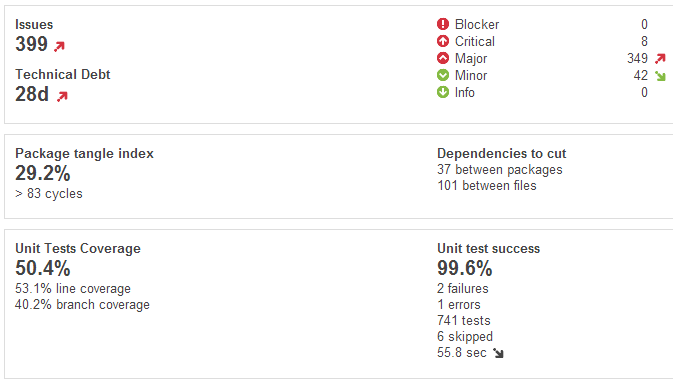
\includegraphics[scale=0.5]{pictures/statistics_group1}

\begin{itemize}
	\item Testing: At the start of the projects, there were no tests written whatsoever. We managed to achieve a 50.4\% coverage. While this is a great step forward, there are still a lot of classes and methods untested, or tests that could be improved. Sometimes it was impossible for us to check a complete class within the scope of the project. This had 2 reasons. Firstly, some methods interact with the \emph{environment}. It wasn't feasible to set up an entire environment to test a simple method. Secondly,  PowerMocking was not possible.

\subparagraph*{PowerMocking}is a system that enables testing of static/ final/private methods. It's a extension of \emph{Mockito} that uses an older version of \emph{java}. While we use the newest version we aren't able to use PowerMocks because of compatibility issues. This makes it impossible to test a lot of the code. 

	\item Issues \& Technical Debt: At this moment there are 399 issues and we have a debt of 28 days. This might sound like a lot, but many of the issues are minor issues, or issues that wrongly marked as an issue.  
	
	\item Decoupling: There are still too many dependencies in the project. There are 37 between packages and 101 between files. This also results in a Package tangle index of	27,6\%  (83 cycles). This is pretty bad and could definitely be improved further.
	
\end{itemize}
	
\subsection*{Strategy}
\begin{itemize}
	\item Testing: Start with looking for a way to create an simple testing \emph{environment} to test the big classes like \emph{server} and \emph{client}. Also try to get PowerMock running (by waiting until it becomes compatible, or finding another method). Make sure to continue testing! 
	\item Issues \& Technical Debt: Issues are divided in Blocker, Critical, Major, Minor and Info. Make sure there are no Blocker and Critical issues and and resolve Major ones that can be fixed. This way you'll not waste too much time fixing issues compared to extending the code.  
	\item Decoupling: With \emph{Sonar} and \emph{Stan} you can visualize the dependencies. When you have an overview you can decide whether to change the class/package and try to cut dependencies. Most likely, restructuring will be needed. 
\end{itemize}

\section{Environment Store}

We think that the software we created can be easily extended in general to include more features, because of the massive effort to restructure the code and to create a framework for features. Aside from the functionalities which we didn't implement, ideas for a new version (which would be BW4T4) could be: more zones (such as repair zones for robots that are damaged by a collision), more hazards in the map that do different things (such as a supercharge zone, which overcharges robots that use a battery and damages them because of the overcharge, but robots without a battery would be unaffected), et cetera. A usability feature would be a button to randomize both the rooms and the block sequence at once, so that the map is still completable, because during the user tests there was a comment that randomizing both the rooms and the blocks/sequence was a little bit of a hassle. This would add more customization to the BW4T environment, and make it more user friendly, allowing it to be a better platform to test out GOAL agents that are going to be used in real life situations, the goal for developing the BW4T environment further. \\

We also made some errors with developing the software. For example, the option to load a map is not in the size dialog but in the map editor. This causes problems because the size of the map is already defined by then, and loading a map of a different size causes the obvious problems, especially when loading a map that is too big. It is also not logical to define the size of the map again before loading the map in the editor. Also, the bot store part of the system does not use the MVC design pattern anymore. It actually did after we refactored its code, but because group 3 was building their parts of the system around the old, non-MVC version of the bot store and we discovered this a day before the deadline, we decided that we would reset the bot store to the non-MVC compliant version. A true shame, but it was necessary because it was only shortly before the deadline and we had way too little time to fix and test everything. Better communication could have helped us here tremendously, but alas. A design issue for a new development group is therefore to recreate the bot store to an MVC compliant part of the system, and also rebuild the environment store to work with this new version.

\subsection*{Wishes from test users}
These are the wishes our participants expressed during the user tests.

\begin{itemize}
\item A one-click-random. It should be possible to randomize everything (zones, blocks and sequence) with one button. The result should be a solvable map, so the randomize functions should take each others' results into account. For example: there cannot be a color in the sequence which does not exist somewhere in a room.
\item Setting more zones at once. It should be possible to select multiple zones by dragging your mouse over them and then changing them all at once into rooms, blockades etc. This would be especially useful when having maps with a lot of zones. 
\item Being able to save a map without it having a start- and drop-zone. 
\item Being able to add parameters to the randomization of both the blocks and map. Example: different odds for reclassifying rooms as blockades/charge zones/corridors, a new probability that a corridor will be reclassified as a charge zone, and a different ratio (relatively) for every possible block color (the probabilities for the map randomization are hardcoded, as well as the ratios for each possible block color).
\end{itemize}

\section{HumanPlayer GUI}
In the current setup of the BW4T environment blocks can be dropped outside a room, but will then disappear from the screen. The environment doesn't provide functions for showing, picking up and communicating about blocks outside rooms. Keeping the visual aspect of the blocks outside a room is a fairly easy fix, implementing the needed functionality to be able to pick blocks back up and communicate about these blocks asks for bigger changes throughout BW4T. \\

The messaging system of the current BW4T environment only allows robots to communicate the most basic commands like the color of a block or the location of a robot. This also means robots are only able to carry out basic tasks. Adding more advanced messages opens up a wide variety of possibilities for more advanced tasks for bots.

At the moment e-partners are displayed as yellow triangles. These could be replaced with an image that represents the function the e-partner has, as this would make it easier for the human player to identify the function of an e-partner.
\section{Path Planning}
In the BW4T environment robots plan their path by navigating through the zones on the map. The navigation algorithm creates a graph consisting of all zones, and calculates the shortest path from the start zone to the destination zone. Each zone has a location on the map, however, this location specifies where the center of the zone is. As a result, when paths are calculated using the zones location, the path always goes through the center of the zone. \\
The new version of BW4T includes collision detection and obstacle avoidance. When navigating around obstacles a new path planner is used, which unlike the usual path planner does not navigate over zones, but points (coordinates) on the map. Due to the higher precision the robot can easily navigate around obstacles in its way. The downside of this path planner is that the algorithm is computationally expensive. A graph with $N$ vertices and up to $N^4$ has to be generated, with N being the product of the width and height of the map (in points). As such the path planner can not be used often as it would significantly slow down the simulation. \\
Since the paths by the original path planner all go through the center of zones, the chance is fairly high that a robot will collide with another bot. While this can be safely navigated, it does not realistically simulate a corridor where more than one bot can concurrently pass through. Due to time constraints this problem remains unsolved, but three possible solutions will be presented. \\

The first solution is to, when planning a path through the zones, return a random point in the zone as opposed to the center of the zone. Because each bot will (most likely) have a different path, collisions will be avoided to an extent. The disadvantage of this method is that the paths will not be elegant. A bot may have to make like a snake to go to a location when a straight line would have been more adequate. Especially with the addition of the battery, which is used when the bot is moving, this may result in an inaccurate simulation of battery use since the bot would be using more energy than is strictly needed. \\
The second solution, albeit more complicated to implement, is to select a random point in the zone, and make sure that the points selected in all subsequent zones have (if possible) either the same X coordinate or Y coordinate. This would result in straighter lines, lowering the battery use and reducing the chance of collisions when criss-crossing between zones. \\
The third solution is to change change the way robots navigate through the map. By only planning a small part of the path at a time and taking other robots into consideration while planning its path a robot could find the shortest possible path to its destination. This however comes with a downside as it could consume a lot of computation power and slow down the simulation.

\section{Final Word}
All in all, there are few things that the customer really wanted but we didn't implement because they had a lower priority than other features. Also, the time given for the project was too short to implement all these features. The things that we didn't implement are the communication handicap (being able to communicate with another bot or not, or having a set chance that a certain message is going to be delivered) because this was too hard to do given the communication of GOAL-programmed agents, and the path finding and collisions of robots (robots can or cannot walk over each other in a path), because this was hard to do and we had time constraints. These are functionalities that can be added by new teams further developing the software. Also, the way we created handicaps allows for easy extension to more handicaps, although some old code had to be rewritten in order to pass the data to the data object and actually be able to see the handicaps in action.
